\section{Analysis strategy}\label{sec:kaonAnalysis} 
 
In this section, we will give an overview of the $K^{+}$-Ar total cross-section analysis strategy. 
The strategy can be summarize in 3 steps:
\begin{itemize}
\item[1.] Identification of kaon candidates in the beam line.
\item[2.] Application of the ``thin-slice'' method.
\item[3.] Identification and treatment of the slices containing a decaying kaon.
\end{itemize}

\subsection{Identification of Kaons in the beam line}

These candidates constitute the pool of events used for the cross section measurement.

\label{sec:BeamlineKStrategy}
\subsection{The thin-slice method}
\label{sec:KXSStrategy}
\subsubsection{Cross Section on Thin Target}\label{sec:thinTargetXS}
Interaction cross sections on thin target are a classic nuclear physics measurement with a well established methodology. A thin target is a target formed by a slab of material containing many uniformly distributed diffusion centers, where  one center is not sitting in front of another.
A pictorial representation of a thin slice experiment is shown schematically in Figure \ref{fig:thinslice}

\begin{figure}[htb]
\centering
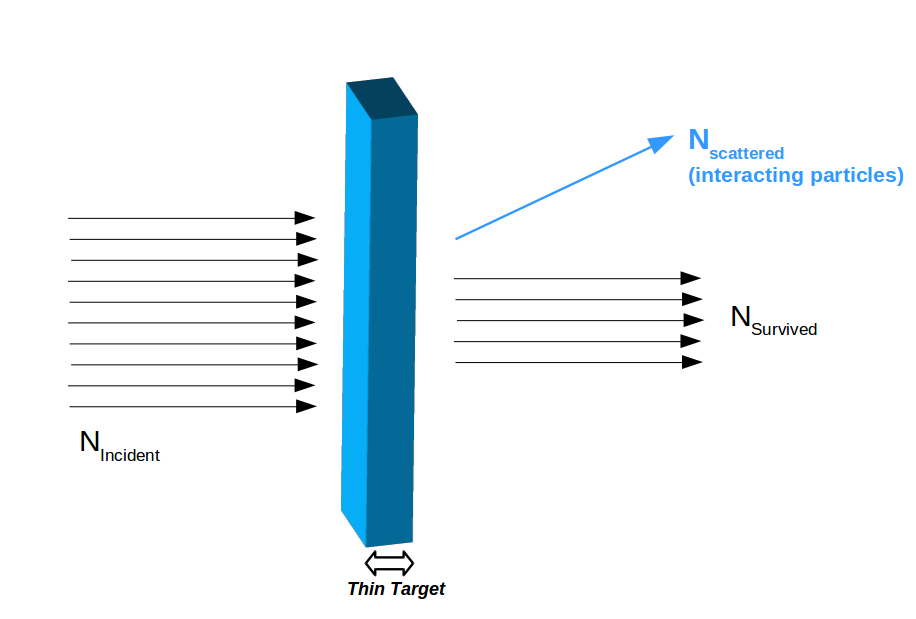
\includegraphics[scale=0.25]{./images/ThinTarget.png}
\caption{Representation of the thin target approximation as a ``thin slice'' of argon experiments.}
\label{fig:thinslice}
\end{figure}

 The survival probability of a kaon traveling through a slab of argon of depth {\it z} and density {\it n} is given by:

\begin{equation}
P_{surv} = e^{-\sigma_{tot}n z}
\end{equation} 
where $\sigma_{tot}$ is the total cross section per nucleon (in $cm^2$), {\textit
{z}} is the target thickness (in cm) along the incident kaon direction, and {\textit
{n}} is the scattering center density in the target, $n=\frac{\rho N_{A} }{A}$ (in $cm^{-3}$). The interaction probability is then $P_{int} = 1 - P_{surv}$. $P_{int}$ is experimentally measured as the ratio of the number of interacting kaons $N_{int}$ over the number of incident kaons $N_{inc}$:
\begin{equation}
P_{int}=\frac{N_{int}}{N_{inc}}=1-e^{-\sigma_{tot}n z}.
\end{equation}

In practices, this assumption of thin target holds true if the target is several order of magnitude smaller than the interaction length. Mathematically speaking, this assumption implies $z\rightarrow\delta z$. Thus, it is possible to Taylor expand the exponential and  solve for the total cross section as a function of energy, $\sigma_{tot}(E)$:
\begin{equation}\label{calc_sigma1}
\frac{N_{int}}{N_{inc}}=1-e^{-\sigma_{tot}n z}\simeq 1-(1-\sigma_{tot}n\delta z + o(\delta z^2)) 
\end{equation}
\begin{equation}\label{calc_sigma2}
\sigma_{tot}(E) \simeq \frac{1}{n\delta z} \Big(\frac{N_{int}}{N_{inc}}\Big) \text{ 	when $z\rightarrow\delta z$}.
%N_{int}(z,E)=(1-N_{inc}e^{-\sigma_{tot}(E)nz})
\end{equation}

In order to measure the cross section, a thin target experiment would simply count the number of incident kaons and the number of surviving kaons.

\subsubsection{Not-so-thin target: sliced TPC}
\label{sec:thick}
The LArIAT TPC, with its 90-cm thick active volume, is not a thin target. Nevertheless, the combination of fine-grained tracking and precise calorimetric information allow us to treat the active volume as a sequence of 240 adjacent thin targets. This technique, called the ``sliced TPC" method, allows to measure the kaon cross section as a function of energy.  In LArIAT, the two wire planes are each made of 240 wires oriented at +/- $60^{\circ}$ with a wire pitch of 4 mm; these planes collect signals proportional to the energy loss of the kaon in a $60^{\circ}$-inclined 4~mm thin slab of liquid argon. Thus, one can think of the TPC as being divided into $\sim$240 slices along the direction of the incident particles ({\textit
{z}} axis) with a spacing $\Delta${\textit
{z}} = 4 mm/sin($60^{\circ}$) $\approx$ 4.5~mm, as shown in Fig.~\ref{fig:slicedtpc}. 
Each slice can be now considered an independent ``thin target" experiment and the cross section calculation in Eq. \ref{calc_sigma2} can be iteratively applied. The kinetic energy of the kaon entering the TPC is determined by measuring its momentum with the tertiary beamline and assuming the kaon mass as mass hypothesis. At each given slice, the kaon incident kinetic  is then determined by subtracting its calorimetric energy released in the previous slice from the total kinetic energy at that slice. Thus, it is possible to perform a differential cross section measurement as a function of the energy because the kaon kinetic energy $K.E._{slice}$  is known before entering each slice. \\ 
When the kaon enters a slice, it contributes to $N_{inc}$ for the energy bin corresponding to  its kinetic energy  that slice. If it interacts in the slice, it also contributes to $N_{int}$ in the appropriate energy bin. If it does not interact, the kaon proceeds to the next slice and the counting is repeated for its new kinetic energy.\\

The uncertainty for each energy bin is calculated by error propagation from the uncertainty on $N_{incident}$ and $N_{interacting}$. 
Since the number of incident pions in each slice is given by a simple counting, it is safe to assume that $N_{incident}$ is distributed as a poissonian with mean and $\sigma^2$ equal to $N_{incident}$ in each bin.  
On the other hand, $N_{interacting}$ follows a binomial distribution: the particle in a given energy bin might or might not interact.  The interaction probability $p$ is $\frac{ N_{interacting}}{N_{incident}}$ and the number of tries $n$ is $N_{incident}$. 
So, the square of the variance for the binomial is given by  $$\sigma^2 = np(1-p) =  N_{incident}\frac{ N_{interacting}}{N_{incident}} (1-\frac{ N_{interacting}}{N_{incident}}) = N_{interacting}(1-\frac{ N_{interacting}}{N_{incident}}).$$

$N_{incident}$ and $N_{interacting}$ are not independent.
The uncertainty on the cross section is thus calculated as 
\begin{equation}
\delta\sigma_{tot}(E) = \sigma_{tot}(E) \Big(\frac{\delta N_{interacting}}{N_{interacting}}+\frac{\delta N_{incident}}{N_{incident}}\Big) 
\end{equation}
where:
\begin{eqnarray}
\delta N_{incident} = \sqrt[]{N_{incident}} \\
\delta N_{interacting} = \sqrt[]{N_{interacting}(1-\frac{ N_{interacting}}{N_{incident}})}.
\end{eqnarray}

%\textcolor{blue}{Sketch of sliced tpc technique?}
\begin{figure}[htpb]
\centering
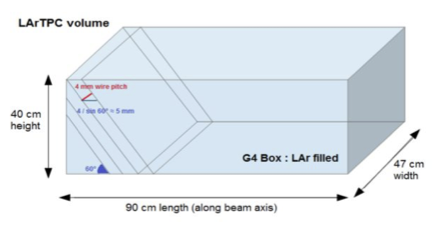
\includegraphics[scale=1.25]{images/Lariat/SlicedTPC.png}\\
\caption{Sketch of Sliced TPC approach.}
\label{fig:slicedtpc}
\end{figure}

It is worth noticing an important difference between the procedure utilized by LArIAT to measure the total hadronic kaon cross section and the procedure used by other experiments in neutrino cross section measurements. In the latter, one needs to correct for the detector inefficiency in identifying neutrinos. In our measurement,  we need do not need to efficiency correct for the beam line candidates which we are not able to identify in the TPC. This is because the cross section calculation in Eq. \ref{calc_sigma2}  relies on measuring the ratio $\frac{ N_{interacting}}{N_{incident}}$, where both these numbers are drawn from tracked kaons in the TPC.


The sliced TPC technique was tested by comparing the results of this method with the prediction of the total hadronic interaction cross section ($K^{+}$, Ar) for thin-target simulations of the Geant 4.10.1 with Bertini Cascade model~\cite{geant4, g4bert}.
Fig.~\ref{fig:xsplot} shows the resulting total ${K^+}$ cross section extracted by the sliced TPC technique; it agrees well with the Geant 4 thin-target cross section.  The comparison of the Geant4 thin- and thick-target cross section results demonstrates the power of the sliced TPC method for the measurement of the ($K^{+}$, Ar) cross section in LArIAT TPC geometry. 

\begin{figure}[h!]
\centering
%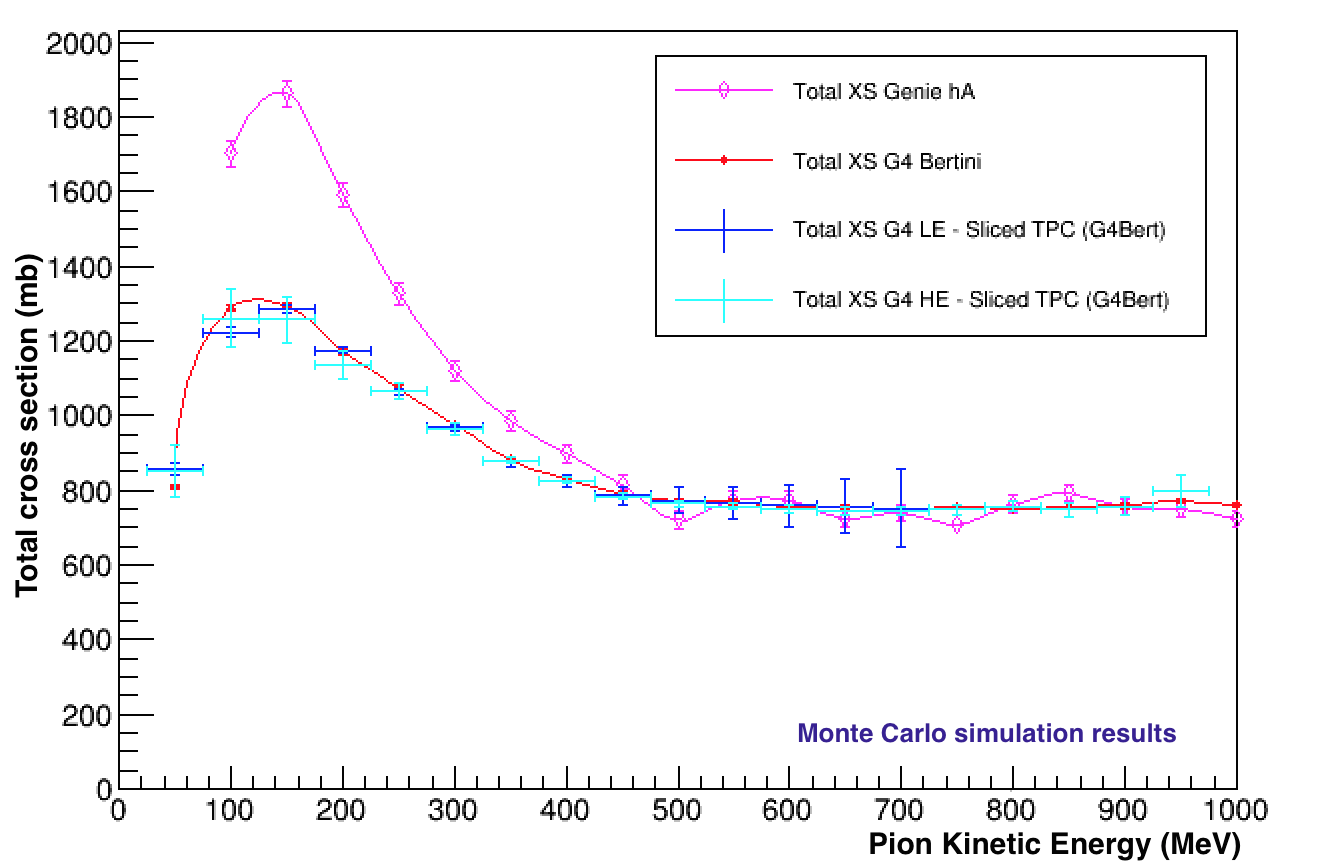
\includegraphics[scale=0.45]{./images/compare_new.png}
\caption{$K^+$ on Ar total cross section dependence on the kinetic energy from MC simulations: comparison between the Geant4 prediction for a LAr thin target and cross section measurement with the sliced TPC technique based on MC truth energy deposited.}
\label{fig:xsplot}
\end{figure}

Having validated the ``Sliced TPC'' technique by showing that it recovers the simulated cross-section, we now move to performing this measurement utilizing the complete LArIATSoft simulation suite.  Furthermore, we move from utilizing truth level MC information to performing fully automated reconstruction of the charged kaon events in the TPC. 



\subsection{Slices containing decays}
We address here an important difference between the thin target and the thick target experiments. While the faction of kaon decay in the thin target is negligible, both in flight and at rest decays play an important role in the thick target case. 
Kaon decay proceeds by the weak interaction; since our goal is to measure the hadronic cross section, slices containing decaying kaons must not contribute to the number of interacting kaons. If one only considers the endpoint of the primary kaon track without identification of the decay, this slice will be wrongly contribute to the $N_{interacting}$ counting. 
In case of kaon decay at rest, the kinetic energy is ideally zero, s shown in figure \textcolor{red}{ADD INTERACTION FIGURE!!!!}. A bragg peak towards the end of the kaon track is also formed as the kaon comes to a stop. A simple way to eliminate the contribution from slices containing kaon decay at rest is putting a lower bound to the energy range of the cross section. We decide to measure the cross section in the region between 100 MeV to 2000 MeV.

Kaon decay in flight are more tricky, since they can happen at any energy. A distinction between interaction and decay is thus needed. 





 Kaon decay tagging is discussed the next section. 




